\documentclass[twoside,twocolumn]{jsarticle}
\usepackage{outline-ec}
\usepackage{amsmath,amssymb,verbatim,ascmac,multicol}
\usepackage{tabularx}
\usepackage[dvipdfmx]{graphicx,color}

\makeatletter
\long\def\@makecaption#1#2{
\sbox\@tempboxa{#1 \hskip0.5zw #2}
\ifdim \wd\@tempboxa >\hsize
#1 #2\par 
\else
\hb@xt@\hsize{\hfil\box\@tempboxa\hfil}
\fi}
\makeatother
\氏名{平田 蓮}
\出席番号{24}
\研究室名{制御工学研究室}
\指導教官{外山}
\発表番号{C\;--\;4}
\研究題目{メタ認知獲得を促進する手軽な運動再現システム}
\研究副題{}
\アブストラクト{
	本研究は、情報端末の内蔵カメラのみを用いて
	スポーツの映像から選手の動きをデータ化し、
	選手の能力向上に貢献することを目的としている。
	現時点では、選手の位置を追跡・再現可能なシステムが完成した。
	最終的には選手の姿勢を再現可能にし、選手の練習による動作の変化の検証及び、
	選手が自身の動きを見直し練習することによるメタ認知獲得促進を目指す。 
}
\begin{document}
\maketitle
\section{研究背景・目的}
	現在、スポーツトレーニングの現場では、
	従来の熟練した指導者の経験に基づく感覚的な指導ではなく、
	科学的に選手の動きを分析して改善する定量的な指導が求められている。
	実際に、バレーボール業界では、イタリア発祥の「データバレー」
	と呼ばれる解析ソフトが実用化されている。
	これを用いアナリストが試合を通して情報の手入力を行うことで、
	選手がコートのどの位置でどのようなプレイをしたか後から見直せる。
	しかし、手入力の練習が必要であること、人為的な入力ミスなど、
	問題点がいくつかあげられる。

	そこで本研究では、バレーボールの試合中の選手の動きのうち、
	特に選手の位置に注目し、人の手を介さない解析を目指す。
	バレーボールの試合映像から試合中の選手のコート上での位置を推定・追跡する。 
	これは現在モーションキャプチャーを用いることで実現可能であるが、
	高価な機器や複雑なキャリブレーションが必要なため、
	実際の試合や練習での利用は難しい。
	そこで、本研究では情報端末の内蔵カメラのみでこれを実現する。 
\section{研究内容・方法}
	選手の位置を推定するにあたってカメラから見たコートの位置情報が必要であるが、
	これは一般的に図\ref{fig:calibration}に示すような基準グリッドを適当に設置し行う
	キャリブレーションを要する。このキャリブレーションを毎回行うのは、
	練習や試合の様子を撮影するにあたって不便である。そのため、
	本研究ではコートのネットに設置してあるアンテナが両方写っている映像を用い、
	各フレーム内でのそれらの位置からコートの全体像及び選手の位置推定を行う。 

	詳しい研究内容をアンテナの検出と人物の推定の二つに分けて以下に述べる。 

	\begin{figure}[h]
		\centering
		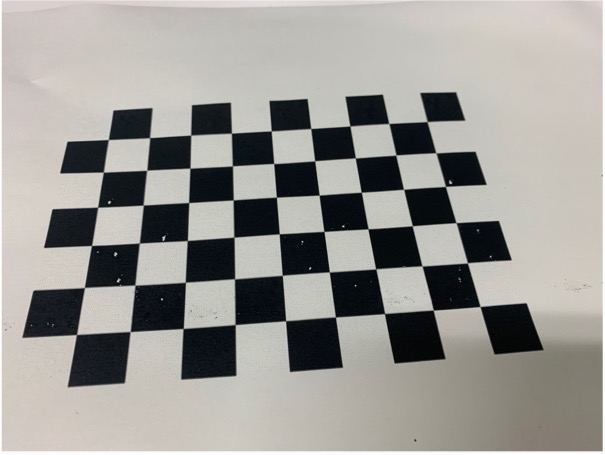
\includegraphics[width=0.8\hsize]{calibration.jpg}
		\caption{キャリブレーションに用いる基準グリッド}
		\label{fig:calibration}
	\end{figure}

	\subsection{アンテナの検出}
		映像内でアンテナの位置を検出するのに、YOLO\cite{Redmon}を用いる。
		SSD\cite{Liu}を用いた開発にも挑戦したが、こちらは最終更新が5年前で、
		現行の周辺ソフトウェアのバージョンと互換性がないため、前者を用いた。

		YOLOを用いると映像内の物体の位置とその物体が何であるかが検出できる。
		今回は検出された物体のうち2本のポールに注目し、
		それぞれの上下端の4点に注目して解析を行なった。

		YOLOの開発者が用意している学習済みモデルを用いると
		アンテナは検出できなかったため、アンテナを含んだデータセットを自作し、
		再学習を行った。
		データセットは適当な背景にアンテナの画像を合わせた画像から成り、
		学習用、検証用それぞれに3000枚ずつ用意した。
		
		詳しい結果は\ref{sec:pole_result}に示す。

	\subsection{選手の位置の推定} \label{sec:pos_theory}
		映像内の選手の位置を検出するのに、AlphaPose\cite{Fang}を用いる。
		上で述べたYOLOなどの物体検知アルゴリズムを用いても映像内の人物の位置推定は
		可能であるが、本研究を発展させて、
		選手の位置だけでなく姿勢の解析も行う際にAlphaPoseによって得られる
		選手の姿勢情報が必要であると考え、これを用いた。

		なお、AlphaPoseで検出可能な距離は、
		コートの端からカメラが約20mの範囲である
		(一般的なスマートフォンのカメラの場合)。 

		アンテナを検出し得られた4点を基準とし、
		AlphaPoseによって得られた映像内の選手の位置に計算を施すことで
		選手の現実世界における座標が得られる。結果を\ref{sec:pos_result}に示す。

\section{研究結果}
	\subsection{ポールの検出} \label{sec:pole_result}
		アンテナの検出に用いた画像及び、アンテナを検出し、
		コートの全体像を推定した様子を図\ref{fig:antenna_original},
		\ref{fig:antenna}に示す。

		\begin{figure}[h]
			\centering
			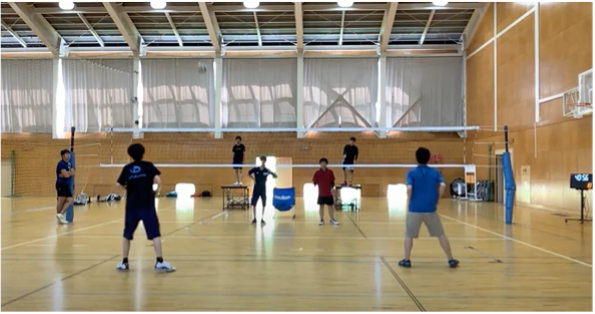
\includegraphics[width=0.8\hsize]{antenna_original.png}
			\caption{アンテナの検出に用いた画像}
			\label{fig:antenna_original}
		\end{figure}

		\begin{figure}[h]
			\centering
			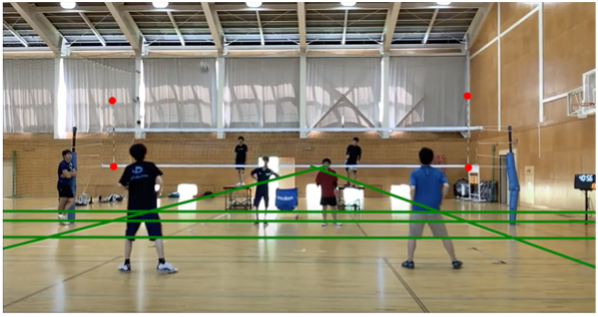
\includegraphics[width=0.8\hsize]{antenna.png}
			\caption{アンテナの検出及びコートライン推定結果}
			\label{fig:antenna}
		\end{figure}

		点で示されているのが前述の4点で、
		直線で示されているのが推定したコートのラインである。
		今回使用したカメラでは正確に検出できている。
		使用するカメラの特性による変化を今後追求検討する。
		もしカメラの特性を考慮しないといけない場合、
		OpenCV\cite{Bradski}などを用いてカメラのパラメータを計測することも
		視野に入れている。

		カメラの特性に作用されないアルゴリズムとして画像内の直線検出があるが、
		一般的な学校の体育館などは複数のスポーツ用にラインが引かれているため、
		今回は使用を見送った。

	\subsection{選手の位置の推定} \label{sec:pos_result}
		図\ref{fig:volley_club},\ref{fig:detection}に位置推定に用いた画像及び、
		それに写っている学生の位置を推定した結果を示す。
		人の目で見る程度ではほぼ正確に位置が推定できているといえる。
		今後、正確に学生の位置を測定した上でどの程度の誤差が発生しているか検証を行う予定である。

		\begin{figure}[h]
			\centering
			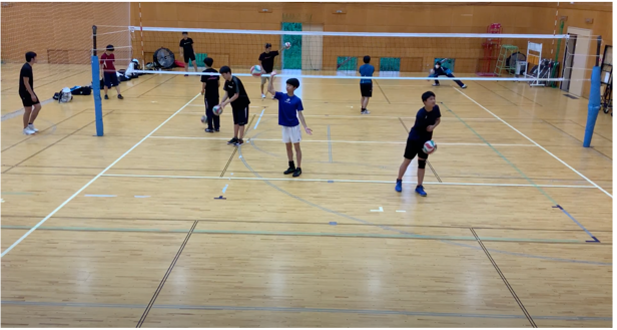
\includegraphics[width=0.8\hsize]{volley_club.png}
			\caption{位置推定に用いた画像}
			\label{fig:volley_club}
		\end{figure}

		\begin{figure}[h]
			\centering
			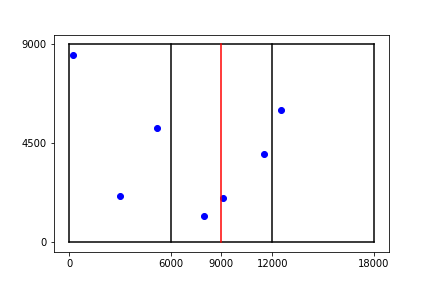
\includegraphics[width=0.8\hsize]{pos.png}
			\caption{学生の位置推定結果}
			\label{fig:detection}
		\end{figure}

		また、今回用いたアルゴリズムでは
		全選手の身長を一定としなければ空中にいる選手に対応することができないため、
		改善方法を探求する必要がある。

\section{まとめ・今後の課題}
	本研究では情報端末の内蔵カメラの映像のみを用いて
	バレーボールのコート内の選手の位置を推定することに成功した。
	これを用いてデータバレーのようなシステムを構築することで
	人為的ミスの余地のないデータ解析を行うことができる。
	今後、位置推定について誤差がどの程度であるか、
	また、精度の上昇につながる測定環境などについて研究を行う。 

	また、今後の研究では、\ref{sec:pos_theory}でも述べたように、
	選手の位置だけでなく姿勢情報を利用し、
	練習や試合の3次元再現を目標とする。

\begin{thebibliography}{99}
	\small{
		\bibitem{Redmon}{
			J. Redmon, S. Divvala, R. Girshick and A. Farhadi,
			``You Only Look Once: Unified, Real-Time Object Detection'',
			2016 IEEE Conference on Computer Vision and Pattern Recognition (CVPR), 2016, pp. 779-788, doi: 10.1109/CVPR.2016.91.
		}
		\bibitem{Liu}{
			Liu W. et al., ``SSD: Single Shot MultiBox Detector'',
			Computer Vision – ECCV 2016. Lecture Notes in Computer Science, vol 9905, 2016
		}
		\bibitem{Fang}{
			Fang Hao-Shu, Xie Shuqin, Tai Yu-Wing and Lu Cewu,
			``RMPE: Regional Multi-person Pose Estimation'',
			ICCV, 2017
		}
		\bibitem{Bradski}{
			Bradski G., ``The OpenCV Library'',
			Dr Dobb's Journal of Software Tools, 2000
		}
	}
\end{thebibliography}
\end{document}
